\documentclass[aspectratio=169,12pt]{beamer}
\usepackage{amsmath}
\usepackage{amssymb}
\usepackage{xcolor}
\usepackage[most]{tcolorbox}
\usepackage{tikz}
\usepackage{graphicx}
\usepackage[sfdefault,lf]{FiraSans}
\renewcommand{\familydefault}{\sfdefault}
\setlength{\parindent}{0pt}
\setbeamertemplate{navigation symbols}{}
\setbeamertemplate{footline}{}
\setbeamertemplate{headline}{}
\definecolor{mmpageWhite}{HTML}{FCFBF7}
\definecolor{mmtanSoft}{HTML}{F7F5EF}
\definecolor{mmgreenDeep}{HTML}{244B2C}
\definecolor{mmgreenLeaf}{HTML}{5D8A56}
\definecolor{mmtext}{HTML}{163221}
\definecolor{mmanswerColor}{HTML}{306A3A}
\setbeamercolor{background canvas}{bg=mmpageWhite}
\setbeamercolor{normal text}{fg=mmtext,bg=mmpageWhite}
\newtcolorbox{AnsCard}[1][]{enhanced,breakable=false,colback=white,colframe=black,boxrule=1.5pt,arc=8pt,left=5pt,right=5pt,top=4pt,bottom=4pt,before skip=0pt,after skip=0pt,height=0.4\textheight,valign=center,#1}
\newcommand{\KoruIcon}{\raisebox{-0.2em}{
\includegraphics[height=1.05em]{img/header-logo.png}}}
\newcommand{\HoeIcon}{\raisebox{-0.2em}{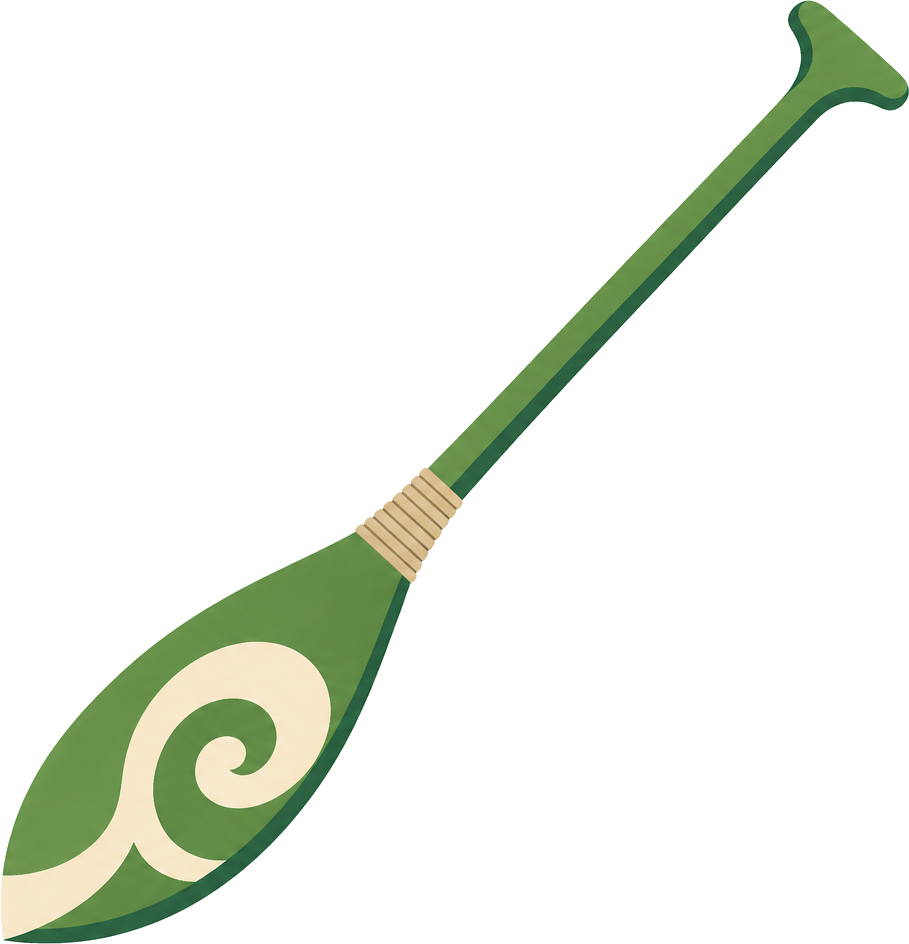
\includegraphics[height=1.05em]{img/hoe.png}}}
\newcommand{\ScaffoldIcons}[1]{\ifcase#1\or \HoeIcon\or \HoeIcon\hspace{0.22em}\HoeIcon\or \HoeIcon\hspace{0.22em}\HoeIcon\hspace{0.22em}\HoeIcon\fi}
\newcommand{\WorksheetTitle}[2]{%
  {\colorbox{mmtanSoft}{\parbox[c][2.2em][c]{0.975\linewidth}{%
    \hspace{0.25em}{\Large\bfseries\textcolor{mmgreenDeep}{#1}\hfill\ScaffoldIcons{#2}}}}
  \par\vspace{0.12em}{\color{mmgreenLeaf}\rule{\linewidth}{2.5pt}}\par\vspace{0.06em}}
}
\setbeamertemplate{background}{
 \begin{tikzpicture}[remember picture,overlay]
 \draw[black,line width=1.5pt,rounded corners=10pt]
 ([xshift=0.45cm,yshift=-0.45cm]current page.north west)
 rectangle
 ([xshift=-0.45cm,yshift=0.45cm]current page.south east);
 \end{tikzpicture}
}
\begin{document}
\begin{frame}[t]
\WorksheetTitle{Push Tasks - Answers}{1}
\vspace{-0.1em}
\begin{columns}[T,onlytextwidth]
\begin{column}{0.48\textwidth}\begin{AnsCard}\small\textcolor{mmgreenDeep}{\textbf{1. Cube side $x$}}\\\vspace{0.1em}\textcolor{mmanswerColor}{\textbf{SA = 6$x^2$}}\end{AnsCard}\end{column}
\begin{column}{0.48\textwidth}\begin{AnsCard}\small\textcolor{mmgreenDeep}{\textbf{2. Prism $l,w,h$}}\\\vspace{0.1em}\textcolor{mmanswerColor}{\textbf{SA = 2(lw+lh+wh)}}\end{AnsCard}\end{column}
\end{columns}
\vspace{0.15em}
\begin{columns}[T,onlytextwidth]
\begin{column}{0.48\textwidth}\begin{AnsCard}\small\textcolor{mmgreenDeep}{\textbf{3. Cube s=6, prism 9$\times$4$\times$h}}\\\vspace{0.1em}\textcolor{mmanswerColor}{\textbf{216=2(36+13h) $\to$ h=72/13 $\approx$ 5.54 cm}}\end{AnsCard}\end{column}
\begin{column}{0.48\textwidth}\begin{AnsCard}\small\textcolor{mmgreenDeep}{\textbf{4. Cuboid 20$\times$10$\times$8}}\\\vspace{0.1em}\textcolor{mmanswerColor}{\textbf{SA = 2(200+160+80) = 880 cm$^2$}}\end{AnsCard}\end{column}
\end{columns}
\vspace{0.15em}
\begin{columns}[T,onlytextwidth]
\begin{column}{0.48\textwidth}\begin{AnsCard}\small\textcolor{mmgreenDeep}{\textbf{5. Open-top box 30$\times$18$\times$12}}\\\vspace{0.1em}\textcolor{mmanswerColor}{\textbf{SA = 1152+540 = 1692 cm$^2$}}\end{AnsCard}\end{column}
\begin{column}{0.48\textwidth}\begin{AnsCard}\small\textcolor{mmgreenDeep}{\textbf{6. Cylinder r=4, h=9}}\\\vspace{0.1em}\textcolor{mmanswerColor}{\textbf{SA $\approx$ 226.08+100.48 = 326.56 cm$^2$}}\end{AnsCard}\end{column}
\end{columns}
\end{frame}
\begin{frame}[t]
\WorksheetTitle{Push Tasks - Answers}{1}
\vspace{-0.1em}
\begin{columns}[T,onlytextwidth]
\begin{column}{0.48\textwidth}\begin{AnsCard}\small\textcolor{mmgreenDeep}{\textbf{7. Cylinder SA=276$\pi$, r=6}}\\\vspace{0.1em}\textcolor{mmanswerColor}{\textbf{12$\pi$h+72$\pi$=276$\pi$ $\to$ h=17 cm}}\end{AnsCard}\end{column}
\begin{column}{0.48\textwidth}\begin{AnsCard}\small\textcolor{mmgreenDeep}{\textbf{8. Square prism s=5, h=12}}\\\vspace{0.1em}\textcolor{mmanswerColor}{\textbf{SA = 2(25)+4(60) = 290 cm$^2$}}\end{AnsCard}\end{column}
\end{columns}
\vspace{0.15em}
\begin{columns}[T,onlytextwidth]
\begin{column}{0.48\textwidth}\begin{AnsCard}\small\textcolor{mmgreenDeep}{\textbf{9. Cube SA=600, find side}}\\\vspace{0.1em}\textcolor{mmanswerColor}{\textbf{6s$^2$=600 $\to$ s$^2$=100 $\to$ s=10 cm}}\end{AnsCard}\end{column}
\begin{column}{0.48\textwidth}\begin{AnsCard}\small\textcolor{mmgreenDeep}{\textbf{10. Compare cuboids}}\\\vspace{0.1em}\textcolor{mmanswerColor}{\textbf{158 vs 164; second greater by 6 cm$^2$}}\end{AnsCard}\end{column}
\end{columns}
\vspace{0.15em}
\begin{columns}[T,onlytextwidth]
\begin{column}{0.48\textwidth}\begin{AnsCard}\small\textcolor{mmgreenDeep}{\textbf{11. Room 6$\times$4.5$\times$2.8, openings 8.2}}\\\vspace{0.1em}\textcolor{mmanswerColor}{\textbf{85.8-8.2 = 77.6 m$^2$}}\end{AnsCard}\end{column}
\begin{column}{0.48\textwidth}\begin{AnsCard}\small\textcolor{mmgreenDeep}{\textbf{12. Can r=3.5, h=12}}\\\vspace{0.1em}\textcolor{mmanswerColor}{\textbf{SA $\approx$ 263.76+76.93 = 340.69 cm$^2$}}\end{AnsCard}\end{column}
\end{columns}
\end{frame}
\begin{frame}[t]
\WorksheetTitle{Push Tasks - Answers}{1}
\vspace{-0.1em}
\begin{columns}[T,onlytextwidth]
\begin{column}{0.48\textwidth}\begin{AnsCard}\small\textcolor{mmgreenDeep}{\textbf{13. Square base 7, SA=238}}\\\vspace{0.1em}\textcolor{mmanswerColor}{\textbf{98+28h=238 $\to$ h=5 cm}}\end{AnsCard}\end{column}
\begin{column}{0.48\textwidth}\begin{AnsCard}\small\textcolor{mmgreenDeep}{\textbf{14. Cube edges double}}\\\vspace{0.1em}\textcolor{mmanswerColor}{\textbf{Factor 2$^2$ = 4}}\end{AnsCard}\end{column}
\end{columns}
\vspace{0.15em}
\begin{columns}[T,onlytextwidth]
\begin{column}{0.48\textwidth}\begin{AnsCard}\small\textcolor{mmgreenDeep}{\textbf{15. Cylinder r,h triple}}\\\vspace{0.1em}\textcolor{mmanswerColor}{\textbf{Factor 3$^2$ = 9}}\end{AnsCard}\end{column}
\begin{column}{0.48\textwidth}\begin{AnsCard}\small\textcolor{mmgreenDeep}{\textbf{16. Cuboid 3:2:1, SA=352}}\\\vspace{0.1em}\textcolor{mmanswerColor}{\textbf{22x$^2$=352 $\to$ x=4 $\to$ 12,8,4}}\end{AnsCard}\end{column}
\end{columns}
\vspace{0.15em}
\begin{columns}[T,onlytextwidth]
\begin{column}{0.48\textwidth}\begin{AnsCard}\small\textcolor{mmgreenDeep}{\textbf{17. Cyl+hemisphere r=3, h=5}}\\\vspace{0.1em}\textcolor{mmanswerColor}{\textbf{30$\pi$+18$\pi$+9$\pi$ = 57$\pi$ $\approx$ 179 units$^2$}}\end{AnsCard}\end{column}
\begin{column}{0.48\textwidth}\begin{AnsCard}\small\textcolor{mmgreenDeep}{\textbf{18. Open cylinder (no top) r=4, h=10}}\\\vspace{0.1em}\textcolor{mmanswerColor}{\textbf{16$\pi$+80$\pi$ = 96$\pi$ $\approx$ 301.44 cm$^2$}}\end{AnsCard}\end{column}
\end{columns}
\end{frame}
\end{document}
